\documentclass[a4paper,oneside,article]{memoir}



% LAYOUT
\usepackage{changepage}
\setulmarginsandblock{0.7\uppermargin}{0.8\lowermargin}{*}

% MATHS
\usepackage{amsmath,amsfonts,amssymb,amsbsy,commath,mathtools,calc}
\mathtoolsset{showonlyrefs,showmanualtags}

\usepackage{subfig}
% FONTS & LANGUAGE
\usepackage[usenames,dvipsnames]{color}
\definecolor{light-gray}{gray}{0.8}
\usepackage{fontspec,xltxtra,polyglossia}
\setmainlanguage{english}
\usepackage[normalem]{ulem} % have underlinings work
%\defaultfontfeatures{Ligatures=TeX}
\defaultfontfeatures{Mapping=tex-text}

\setmainfont[Ligatures={Common}, Numbers={OldStyle}]{Linux Libertine O}
%\setmainfont{Droid Sans}
%\setsansfont[Scale=MatchLowercase]{Inconsolata}
\setmonofont[Scale=0.8]{DejaVu Sans Mono}

% PDF SETUP
\usepackage[unicode,bookmarks, colorlinks, breaklinks,
pdftitle={T-61.5140: Prerequisites},
pdfauthor={Ville Väänänen},
pdfproducer={xetex}
]{hyperref}
\hypersetup{linkcolor=black,citecolor=black,filecolor=black,urlcolor=MidnightBlue} 

% TABLES
\usepackage{booktabs}
\usepackage{topcapt} 
\usepackage{rccol}
\usepackage{tabularx} % requires array
\newcommand{\otoprule}{\midrule[\heavyrulewidth]}
\newcolumntype{d}[2]{R[.][.]{#1}{#2}}

\usepackage{titlesec}

%%%%%%%% OMAT KOMENNOT %%%%%%%%%%%%

\usepackage{mymath}
\usepackage{mylayout}



% PARAGRAPHS
%\usepackage{parskip}

% kuvat

\usepackage{listings}
\usepackage{mcode}
\lstset{ %
	%language=Matlab,                % choose the language of the code
	basicstyle=\footnotesize\ttfamily,% the size of the fonts that are used for the code 
	numbers=none,                   % where to put the line-numbers
	numberstyle=\footnotesize\ttfamily,      % the size of the fonts that are usedfor the line-numbers 
	stepnumber=5,                   % the step between two line-numbers. If it's 1 each line 
	aboveskip=2\medskipamount,
	belowskip=2\medskipamount,                                % will be numbered
	numbersep=-5pt,                  % how far the line-numbers are from the code
	backgroundcolor=\color{white},  % choose the background color. You must add \usepackage{color}
	showspaces=false,               % show spaces adding particular underscores
	showstringspaces=false,         % underline spaces within strings
	showtabs=false,                 % show tabs within strings adding particular underscores
	frame=l,
	framesep=0pt,
	framexleftmargin=2mm,
	rulecolor=\color{light-gray},	                % adds a frame around the code
	tabsize=2,	                % sets default tabsize to 2 spaces
	caption=,
	captionpos=t,                   % sets the caption-position to bottom
	breaklines=true,                % sets automatic line breaking
	breakatwhitespace=false,        % sets if automatic breaks should only happen at whitespace
	emptylines=*1,
	%title=\lstname,                 % show the filename of files included with
	                                % also try caption instead of title
	escapeinside={\%*}{*)},         % if you want to add a comment within your code
            % if you want to add more keywords to the set
}

\newcommand{\course}{S-114.4202}
\newcommand{\coursename}{Special Course in Computational Engineering II}
\newcommand{\duedate}{\today}
\newcommand{\studentid}{63527M}
\renewcommand{\title}{Exercise Report}
\author{Ville Väänänen}

\setsecnumdepth{subsubsection}
\counterwithout{section}{chapter}
%\counterwithout{subsubsection}{section}
%\counterwithout{subsubsection}{subsection}
%\renewcommand\thesection{\arabic{section}}
\checkandfixthelayout
\renewcommand{\thesubsubsection}{\thesubsection{\large\scshape\alph{subsubsection}}}
\newfontfamily\subsubsectionfont[Letters=SmallCaps]{Linux Libertine O}
\titleformat{\subsubsection}{\large\scshape}{\alph{subsubsection} )}{10pt}{}
\titleformat{\section}{\Huge}{Round \thesection}{10pt}{}
\titleformat{\subsection}{\Large}{Exercise \thesubsection}{10pt}{}

\everymath{\displaystyle}
\begin{document}

\begin{titlingpage}
	\begin{adjustwidth}{-0.6in}{-0.6in}
	\begin{center}
		%\begin{minipage}{1.2\textwidth}
			\begin{flushright} \large
			Ville \textsc{Väänänen}\\
			\studentid\\
			ville.vaananen@aalto.fi
			\end{flushright}
		%\end{minipage}
		\vspace{8.0cm}
		
		\textsc{\LARGE \title}
		\HRule \\[0.19cm]
		{\large \course\: \coursename}
		
		\vfill
		\today
	\end{center}
	\end{adjustwidth}
\end{titlingpage}
\newpage


\section{}
\subsection{}
\subsubsection{}

The problem can be written in matrix form as follows:
\begin{align*}
	\v{y} &= \begin{bmatrix} y_1 & \dots & y_n \end{bmatrix}^T \\
	\v{a} &= \begin{bmatrix} a_1 & a_2 \end{bmatrix}^T \\	
	\v{X} &= \begin{bmatrix} 
				x_1 & 1 \\
				\vdots & \vdots \\
				x_n & 1 
%			 \end{bmatrix}^T \\
	\end{bmatrix} \\
	\v{y} &= \v{Xa}
\end{align*}

\subsubsection{}

\begin{align*}
	\mathrm{E}(a_1,a_2)&=(\v{y}-\v{Xa})^T(\v{y}-\v{Xa})
\end{align*}

\subsubsection{}
To compute the LS-estimate $\hat{\v{a}}$, we need to find the global minimum of $\mathrm{E}$, which can be
found by setting its gradient to zero (it's a quadratic form):
\begin{align}
	\nabla\mathrm{E}&=-2\v{X}^T(\v{y}-\v{Xa})\\
	&=2\v{X}^T\v{X}\v{a}-2\v{X}^T\v{y} \\
	\Rightarrow \hat{\v{a}} &= (\v{X}^T\v{X})^{-1}\v{X}^T\v{y}
\end{align}

\subsection{}
\subsubsection{}

The second order differential equation can be written as a first order vector valued differential equation as follows:
\begin{align}
	\dod{\v{x}(t)}{t}&=
	\begin{bmatrix}
	0&-c^2\\
	1&0
	\end{bmatrix}
	\begin{bmatrix}
	x'(t)\\
	x(t)
	\end{bmatrix}
	+
	\begin{bmatrix}
	1\\
	0
	\end{bmatrix}
	w(t)\\
	\Leftrightarrow\v{x}'(t)&=\v{F}\v{x}(t)+\v{L}w(t).
\end{align}
Let us proceed to solve this equation:
\begin{align}
	\v{x}'(t)-\v{F}\v{x}(t)&=\v{L}w(t)\\
	e^{-\v{F}t}\v{x}'(t)-e^{-\v{F}t}\v{F}\v{x}(t)&=e^{-\v{F}t}\v{L}w(t)\\
	\dod{}{t}\left(e^{-\v{F}t}\v{x}(t)\right)&=e^{-\v{F}t}\v{L}w(t)\shortintertext{so that}\\
	\v{x}(t)&=e^{\v{F}(t-t_0)}\v{x}(t_0)+\defint{t_0}{t}{e^{\v{F}(t-s)}\v{L}w(s)}{s} \label{eq:contsol}\shortintertext{where}\\
	\v{x}(t_0)&=
	\begin{bmatrix}
	v_0\\
	x_0
	\end{bmatrix}
\end{align}

\subsubsection{}
% After discretizing the time into $n+1$ instants as $\{t_0=0,t_1=\Delta t,\dots,t_n=n\Delta t\}$
% we can approximate \eqref{eq:contsol} as
% \begin{align}
% 	\v{x}(t_k)=\v{x}(t_{k-1}+\Delta t)&= \v{x}_0e^{\v{F}t_{k-1}}e^{\v{F}\Delta t}+\v{L}\Delta t\sum_{j=1}^{k}e^{\v{F}(t_{k-1}+\Delta t-t_{j-1})}w_{j-1}
% \end{align}
% where we have approximated the integral with its Riemannian sum and $w_{j-1}=w(t_{j-1})$.
% This can be further simplified into
% \begin{align}
% 	\v{x}(t_k)&= e^{\v{F}\Delta t}\left(\v{x}_0e^{\v{F}t_{k-1}}+\v{L}\Delta t\sum_{j=1}^{k-1}\left(e^{\v{F}(t_{k-1}-t_{j-1})}w_{j-1}\right) + \v{L}\Delta tw_{k-1}\right)\\
% 	&=e^{\v{F}\Delta t}\v{x}(t_{k-1}) + \v{L}\Delta t e^{\v{F}\Delta t} w_{k-1}
% \end{align}

After discretizing the time into $n+1$ instants as $\{t_0=0,t_1=\Delta t,\dots,t_n=n\Delta t\}$ and assuming $w(s)=w(t_{k-1})\; \forall s\in[t_{k-1},t_k)$
we can write \eqref{eq:contsol} as
\begin{align}
	\v{x}(t_k)&=e^{\v{F}(t_k-t_0)}\v{x}(t_0)+\sum_{j=1}^k \defint{t_{j-1}}{t_j}{e^{\v{F}(t_j-s)}\v{L}w(s)}{s}\\
	&=e^{k\v{F}\Delta t}\v{x}(t_0)+\sum_{j=1}^k \defint{t_{j-1}}{t_j}{e^{\v{F}(t_j-s)}}{s}\v{L}w(t_{j-1})\\
\end{align}
Now, because the of the constant time intervals, the integral inside the summation is also constant:
\begin{align}	
	&=e^{k\v{F}\Delta t}\v{x}(t_0)+\defint{0}{\Delta t}{e^{\v{F}(\Delta t-s)}}{s}\v{L}\sum_{j=1}^k w(t_{j-1})\\
	&=e^{\v{F}\Delta t}\v{x}(t_{k-1})+\defint{0}{\Delta t}{e^{\v{F}(\Delta t-s)}}{s}\v{L} w(t_{k-1})\\
	&=\v{A}\v{x}(t_{k-1})+\v{B}w(t_{k-1})
	\shortintertext{where}
	\v{A}&=\begin{bmatrix}
		1 & e^{-c^2\Delta t}\\
		e^{\Delta t} & 1
	\end{bmatrix}\\
	\v{B}&=\begin{bmatrix}
		\Delta \\
		e^{\Delta t} - 1
	\end{bmatrix}\\
\end{align}

% After discretizing the time into $n+1$ instants as $\{t_0=0,t_1=\Delta t,\dots,t_n=n\Delta t\}$ and assuming $w(s)=w(t_{k-1})\; \forall s\in[t_{k-1},t_k)$
% we can write \eqref{eq:contsol} for a single interval $[t_{k-1},t_k]$ as
% \begin{align}
% 	\v{x}(t_k)&=e^{\v{F}\Delta t}\v{x}(t_{k-1})+\defint{t_{k-1}}{t_k}{e^{\v{F}(t_k-s)}\v{L}w(s)}{s}\\
% 	&=e^{\v{F}\Delta t}\v{x}(t_{k-1})+\defint{t_{k-1}}{t_k}{e^{\v{F}(t_k-s)}}{s}\v{L}w(t_{k-1})\\
% 	&=e^{\v{F}\Delta t}\v{x}(t_{k-1})+(-\v{F}^{-1})\left(1-e^{\v{F}\Delta t}\right)\v{L}w(t_{k-1})\\
% 	&=e^{\v{F}\Delta t}\v{x}(t_{k-1})+\v{F}^{-1}(e^{\v{F}\Delta t}-1)\v{L}w(t_{k-1})\\
% 	&=\v{A}\v{x}(t_{k-1})+\v{B}w(t_{k-1})\\		
% \end{align}

\subsubsection{}

Assuming $w_{k-1}\sim N(0,\frac{q_c}{\Delta t})$ and $r_{k}\sim N(0,R_k)$ and that at each timestep $t_k$ we measure 
the value of $x(t_k)$ and additive zero mean gaussian noise with variance $R_k$ and designating 
$\v{x}_k=\v{x}(t_{k})$ and $w_k=w(t_{k})$ we get the following linear Gaussian state space model:

\begin{align}
	%\v{x_k}&=\begin{bmatrix} 1 & e^{-c^2\Delta t}\\ e^{\Delta t} & 1 \end{bmatrix}\v{x}_{k-1}+\begin{bmatrix} 0 \\ -c^{-2}\left(e^{-c^2\Delta t}-1\right) \end{bmatrix}w_{k-1}\\
	\v{x}_k&=\v{A}\v{x}_{k-1}+\v{B}w_{k-1}\\
	y_k&=\begin{bmatrix} 0 & 1 \end{bmatrix}\v{x_k}+r_k \shortintertext{so that} \\
	\v{x}_{k}|\v{x}_{k-1} &\sim N\left(\v{A}\v{x}_{k-1},\;\v{B}\frac{q_c}{\Delta t}\v{B}^T\right)\\
	y_{k}|\v{x}_{k} &\sim N\left(\begin{bmatrix} 0 & 1 \end{bmatrix}\v{x}_k,\;R_k \right)   
\end{align}


\subsubsection{}

Assuming $c=0$ we have
\begin{align}
	\v{M}=e^{(\Delta t-s)\v{F}}\v{L}q_c\v{L}^T\left(e^{(\Delta t-s)\v{F}}\right)^T&=
	\begin{bmatrix}
	q_c & q_ce^{\left(\Delta t-s\right)}\\
	q_ce^{(\Delta t-s)} & q_ce^{2\left(\Delta t-s\right)}
	\end{bmatrix}
\end{align}
so that
\begin{align}
	\v{Q}_{k-1}&=\defint{0}{\Delta t}{\v{M}}{s}=
	\begin{bmatrix}
		q_c\Delta t & q_c\left(e^{\Delta t}-1\right)\\
		q_c\left(e^{\Delta t}-1\right) & \frac{q_c}{2}\left(e^{2\Delta t}-1\right)
	\end{bmatrix}
\end{align}
The corresponding covariance matrix in the ZOH discretation case is
\begin{align}
	\v{B}\frac{q_c}{\Delta t}\v{B}^T&=\begin{bmatrix}
		q_c\Delta t & q_c\left(e^{\Delta t}-1\right)\\
		q_c\left(e^{\Delta t}-1\right) & \frac{q_c}{\Delta t}\left(e^{2\Delta t}-2e^{\Delta t}+1\right)
	\end{bmatrix}
\end{align}

\subsection{}\label{sec:1_3}


In this exercise Kalman filtering is practised with the help of the EKF/UKF toolbox.
The results are illustrated in figure~\ref{fig:ex_1_3}, the RMSE values are presented
in table~\ref{table:rmse_1_3} and the m-code is listed in listing~\ref{lst:1_3}.


\begin{figure}[htb]
  \begin{adjustwidth}{-2in}{-2in}
	  \centering
	  \subfloat[First components and
	  measurements]{\label{fig:ex_1_3_signal}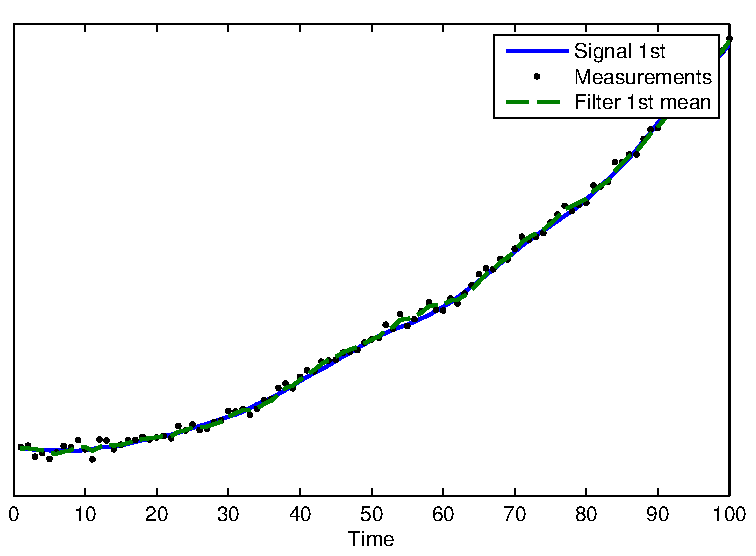
\includegraphics[width=0.7\textwidth]{ex_1_3_signal}}
	  \subfloat[Second components]{\label{fig:ex_1_3_derivative}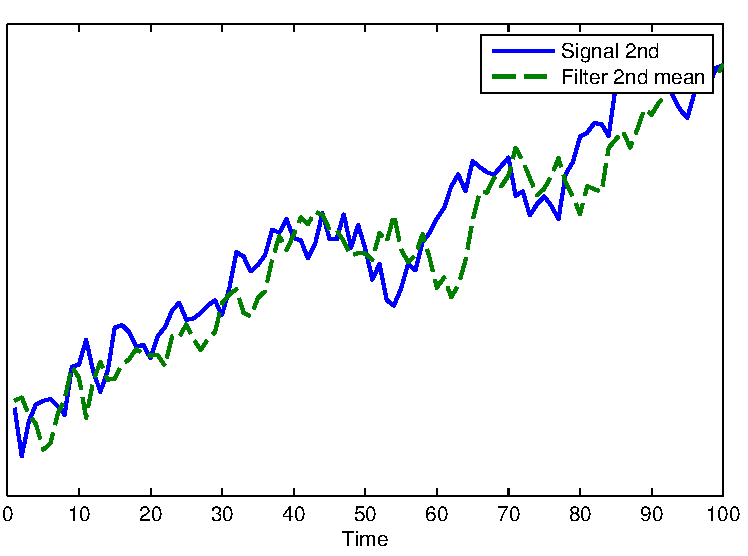
\includegraphics[width=0.7\textwidth]{ex_1_3_derivative}}
  \end{adjustwidth}
  	  \caption{Illustrations of the signal, the measurements and the Kalman filter means in exercise~\ref{sec:1_3}}
	  \label{fig:ex_1_3}
\end{figure}

\begin{table}[h!]
	\centering
	\topcaption{RMSE values for the first component of the signal when the Kalman
	filter means are used as the estimate and when the measuremenst are used as the estimate
	in exercise~\ref{sec:1_3}}
	\begin{tabular}{rd{2}{2}d{3}{2}}
\toprule
&\multicolumn{1}{c}{{\bfseries Filter}}&\multicolumn{1}{c}{{\bfseries Measurements}}\\\otoprule
{\bfseries RMSE}&$60.89257$&$103.11263$\\
\bottomrule\end{tabular}

	\label{table:rmse_1_3}
\end{table} 

\lstinputlisting[caption={m-code in exercise~\ref{sec:1_3}},label=lst:1_3]{ex1_3.m}



\section{}
\subsection{}
\subsubsection{}
The posterior is of the form
\[
p(\v{a}|y_{1:n})=Ze^{f(\v{a})}
\]
where the exponent $f(\v{a})\::\:\R^2\to\R$ can be written as
\begin{align}
	f(\v{a}) &= -\frac{1}{2}\left((\v{Xa}-\v{y})^T(\v{Xa}-\v{y})+\frac{1}{\sigma^2}\v{a}^T\v{a}\right)\\
	&= -\frac{1}{2}\left((\v{a}-\v{m})^T\v{P}^{-1}(\v{a}-\v{m})\right)
\end{align}
with suitably defined mean $\v{m}$ and covariance matrix $\v{P}$. Here $\v{a}$, $\v{X}$ and $\v{y}$ are defined
as in Round 1 exercise 1.


\subsubsection{}
The maximum of the posterior, which also is its mean in this case, is at the maximum of $f(\v{a})$, which can be found 
at the point where its gradient vanishes:

\begin{align}
	\dpd{f(\v{a})}{\v{a}} &= -\v{X}^T(\v{Xa}-\v{y})-\frac{1}{\sigma^2}^T\v{a} = -\left(\v{X}^T\v{X}+\frac{1}{\sigma^2}\v{I}\right)\v{a} + \v{X}^T\v{y}
\end{align}
so that at the maximum $\v{m}$
\begin{align}
	\v{X}^T\v{X}\v{m}+\frac{1}{\sigma^2}\v{m} &= \v{X}^T\v{y} \\
	\v{m} &= \left(\v{X}^T\v{X}+\frac{1}{\sigma^2}\v{I}\right)^{-1}\v{X}^T\v{y} \\
\end{align}

\subsubsection{}

The Hessian matrix of $f$ is

\begin{align}
	\dpd[2]{f(\v{a})}{\v{a}} = -\left(\v{X}^T\v{X}+\frac{1}{\sigma^2}\v{I}\right).
\end{align}
In order to relate this to $\v{P}$, we can calculate that

\begin{align}
	\dpd[2]{}{\v{a}}\left[-\frac{1}{2}\left((\v{a}-\v{m})^T\v{P}^{-1}(\v{a}-\v{m})\right)\right] = -\v{P}^{-1} \label{eq:gauss_hessian}
\end{align}
so that 
\[
	\v{P} = \left(\v{X}^T\v{X}+\frac{1}{\sigma^2}\v{I}\right)^{-1}
\]

\subsubsection{}

The resulting posterior distribution is then

\begin{align}
	p(\v{a}|y_{1:n})&=\mathrm{N}(\v{a}|\v{m},\v{P})\\
	\v{m} &= \v{P}\v{X}^T\v{y}\\ 
	\v{P} &= \left(\v{X}^T\v{X}+\frac{1}{\sigma^2}\v{I}\right)^{-1}
\end{align}
Comparing $\v{m}$ to the LS estimate $\v{m}_{\mathrm{LS}}$ in Round 1 Exercise 1 we can see that
if the prior variance $\sigma^2$ approaches infinity, then $\v{m}\to\v{m}_{\mathrm{LS}}$. 

\subsection{}

The linear regression model in the last exercise can be written in the following state space form

\begin{align}
	\v{a}_k&=\v{a}_{k-1}=\v{a}=\begin{bmatrix} a_1 & a_2 \end{bmatrix}^T \sim N(\v{a}|\v{0},\sigma^2\v{I})\\
	y_k&=\v{H}_k\v{a}+\varepsilon_k,\; k=1,\dots,n \\
	\v{H}_k&=\begin{bmatrix} x_k & 1 \end{bmatrix} \\
	\varepsilon_k &\sim N(\varepsilon_k|0,1)
\end{align}
From these definitions we can deduce that the measurement distribution is
\begin{align}
	p(y_k|x_k,\v{a})=N(y_k|\v{H}_k\v{a},1)
\end{align}
As before, we are interested in the posterior distribution of $\v{a}$. The ``states'' $x_k$ are fixed
and have no associated uncertainty. 

%In the following all the distributions conditioned on $y_{1:k}$ are also implicitely
%conditioned on  $x_{1:k}$. 

\subsubsection{}

After the first observation we have

\begin{align}
	p(\v{a}|y_1,x_1)&=\frac{p(y_1|x_1,\v{a})p(\v{a})}{p(y_1|x_1)}
\end{align}
Now noting that $p(\v{a})=N(a_1|0,\sigma^2)N(a_2|0,\sigma^2)$ and designating $Z=p(y_1|x_1)^{-1}$, 
we find that this distribution is exactly the same as the posterior in the previous exercise with $n=1$.
Similarly after $k\leq n$ measurements we get (the measurements are considered i.i.d)
\begin{align}
	p(\v{a}|y_{1:k},x_{1:k})&=\frac{\prod_{j=1}^k p(y_j|x_j,\v{a})p(\v{a})}{p(y_{1:k}|x_{1:k})}.
\end{align}
that is again the same as the posterior in the previous exercise with $n=k$.

We can then use the results from the last exercise by replacing $n$ with $k$ in the equations. If we designate by 
$\v{X}_k$ and $\v{y}_k$ the $\v{X}$ and $\v{y}$ of the previous exercise but with $k$ instead of $n$ elements and with $\v{m}_k$ and 
$\v{P}_k$ the mean and covariance matrix of the posterior after $k$ measurements,
we get

\begin{align}
	\v{m}_k &= \v{P}_k\v{X}^T_k\v{y}_k \label{eq:regression_batch_mean}\\
	\v{P}_k&= \left(\v{X}_k^T\v{X}_k+\frac{1}{\sigma^2}\v{I}\right)^{-1}\\
\end{align} 

\subsubsection{}

For the covariance matrix we can write
\begin{align}
	\v{X}_k^T\v{X}_k &= 
	\begin{bmatrix}
		\sum_i^kx_i^2 & \sum_i^kx_i \\
		\sum_i^kx_i & k   
	\end{bmatrix}\\
	\v{H}_k^T\v{H}_k &= 
	\begin{bmatrix}
		x_k^2 & x_k \\
		x_k & 1   
	\end{bmatrix}\\
	\Leftrightarrow \v{X}_k^T\v{X}_k &=\v{X}_{k-1}^T\v{X}_{k-1}+\v{H}_k^T\v{H}_k  
\end{align}
giving
\begin{align}
	\v{P}_k&= \left(\v{X}_{k-1}^T\v{X}_{k-1}+\v{H}_k^T\v{H}_k+\frac{1}{\sigma^2}\v{I}\right)^{-1}.
\end{align}
Similarly for the mean we get
\begin{align}
	\v{X}_k^T\v{y}_k &= 
	\begin{bmatrix}
		\sum_i^kx_iy_i \\
		\sum_i^ky_i   
	\end{bmatrix}\\
	\v{H}_k^Ty_k &= 
	\begin{bmatrix}
		x_ky_k \\
		y_k & 1   
	\end{bmatrix}\\
	\Leftrightarrow \v{X}_k^T\v{y}_k &=\v{X}_{k-1}^T\v{y}_{k-1}+\v{H}_k^Ty_k  
\end{align}
giving
\begin{align}
	\v{m}_k&= \v{P}_k\v{X}_{k-1}^T\v{y}_{k-1}+\v{P}_k\v{H}_k^Ty_k \label{eq:mean_xk1}
\end{align}


\subsubsection{}

Let's start by substituting first $\v{K}_k$ and then $\v{S}_k$ into $\v{P}_k$

\begin{align}
	\v{P}_k &=\v{P}_{k-1}-\v{P}_{k-1}\v{H}_k^T\v{S}_k^{-1}\v{S}_k\v{S}_k^{-1}\v{H}_k\v{P}_{k-1}&\\
	&=\v{P}_{k-1}-\v{P}_{k-1}\v{H}_k^T\left( \v{H}_k\v{P}_{k-1}\v{H}_k^T+1 \right)^{-1}\v{H}_k\v{P}_{k-1}\label{eq:variance_long}\shortintertext{apply the matrix inversion lemma}
	&= \left( \v{P}_{k-1}^{-1} +\v{H}_k^T\v{H}_k \right)^{-1}\\
	&=\left( \v{X}_{k-1}^T\v{X}_{k-1}+\frac{1}{\sigma^2}\v{I}+\v{H}_k^T\v{H}_k \right)^{-1}\\
	&=\left( \v{X}_{k}^T\v{X}_{k}+\frac{1}{\sigma^2}\v{I} \right)^{-1}	
\end{align}

\subsubsection{}

In part b) it was proved that the result in part a) can be written as in \eqref{eq:mean_xk1}. 
By using the identities
$\v{K}_k=\v{P}_k\v{H}_k^T=\v{P}_{k-1}\v{H}_k^T \left( \v{H}_k\v{P}_{k-1}\v{H}_k^T+1 \right)^{-1}$
this can be derived from the Kalman filter equations: 

\begin{align}
	\v{m}_k&= \v{m}_{k-1} + \v{K}_k(\v{y}_{k}-\v{H}_k\v{m}_{k-1})\\
	&=\left(\v{I}-\v{K}_k\v{H}_k\right)\v{m}_{k-1}+\v{K}_k\v{y}_{k}
	\shortintertext{apply equation \eqref{eq:regression_batch_mean}}
	&=\left(\v{I}-\v{K}_k\v{H}_k\right)\v{P}_{k-1}\v{X}_{k-1}^T\v{y}_{k-1}+\v{K}_k\v{y}_{k}\\
	&=\left(\v{P}_{k-1}-\v{K}_k\v{H}_k\v{P}_{k-1}\right)\v{X}_{k-1}^T\v{y}_{k-1}+\v{K}_k\v{y}_{k}
	\shortintertext{apply the identities}
	&=\left(\v{P}_{k-1}-\v{P}_{k-1}\v{H}_k^T \left( \v{H}_k\v{P}_{k-1}\v{H}_k^T+1 \right)^{-1}\v{H}_k\v{P}_{k-1}\right)\v{X}_{k-1}^T\v{y}_{k-1}+\v{P}_k\v{H}_k^T\v{y}_{k}
	\shortintertext{apply equation \eqref{eq:variance_long}}
	&=\v{P}_k\v{X}_{k-1}^T\v{y}_{k-1}+\v{P}_k\v{H}_k^Ty_k
\end{align}

\subsubsection{}

\begin{itemize}
  \item step 1
  \begin{itemize}
  	\item mean
\begin{align}
	\v{m}_{0}&=0\\
	\v{P}_0&=\sigma^2\v{I}\\
	\Leftrightarrow \v{m}_{1}&=\v{m}_{0}+\v{P}_1\v{H}_1^T(\v{y}_{1}-\v{H}_1\v{m}_{0})\\
	&=\v{P}_1\v{X}_1^T\v{y}_{1}
\end{align}
  	\item variance 
\begin{align}
	\v{P}_{1}&= \left(\v{X}_1^T\v{X}_1+\v{P}_{0}^{-1}\right)^{-1}
\end{align}
  \end{itemize}
  \item step k
  \begin{itemize}
  	\item mean (assume $\v{m}_{k-1}= \v{P}_{k-1}\v{X}_{k-1}^T\v{y}_{k-1}$)
\begin{align}
	\v{m}_{k}&=\v{m}_{k-1} + \v{K}_k(\v{y}_{k}-\v{H}_k\v{m}_{k-1})\\
	&=\v{P}_k\v{X}_{k-1}^T\v{y}_{k-1}+\v{P}_k\v{H}_k^Ty_k\\
	&=\v{P}_k\v{X}_{k}^T\v{y}_{k}
\end{align}
  	\item variance (assume $\v{P}_{k-1}= \left(\v{X}_{k-1}^T\v{X}_{k-1}+\v{P}_{0}^{-1}\right)^{-1}$)
\begin{align}
	\v{P}_{k}&= \left( \v{P}_{k-1}^{-1} +\v{H}_k^T\v{H}_k \right)^{-1}\\
	&=\left( \v{X}_{k-1}^T\v{X}_{k-1}+\v{P}_{0}^{-1}+\v{H}_k^T\v{H}_k \right)^{-1}\\
	&=\left( \v{X}_{k}^T\v{X}_{k}+\v{P}_{0}^{-1} \right)^{-1}	
\end{align}
  \end{itemize}
\end{itemize}

\subsection{}

\subsubsection{}

\begin{align}
	p(\v{x})&=N(\v{x}|\v{m},\v{P}),\;\v{x}\in\R^n\\
	p(\v{y}|\v{x})&=N(\v{y}|\v{H}\v{x},\v{R}),\;\v{y}\in\R^m\\
	\Leftrightarrow p(\v{x},\v{y})&=p(\v{y}|\v{x})p(\v{x})\\
	&=C\exp\left(-\frac{1}{2}(\v{x}-\v{m})^T\v{P}^{-1}(\v{x}-\v{m})-\frac{1}{2}(\v{y}-\v{H}\v{x})^T\v{R}^{-1}(\v{y}-\v{H}\v{x})\right)\\
	&=C\exp\left(-\frac{1}{2}
	\begin{bmatrix}
		\v{x}-\v{m}\\
		\v{y}-\v{H}\v{m}
	\end{bmatrix}^T
	\begin{bmatrix}
		\v{P}&\v{P}\v{H}^T\\
		\v{H}\v{P}&\v{H}^T\v{P}\v{H}+\v{R}
	\end{bmatrix}^{-1}
	\begin{bmatrix}
		\v{x}-\v{m}\\
		\v{y}-\v{H}\v{m}
	\end{bmatrix}
	\right)
\end{align}
Now from the last form we can see that the joint distribution is clearly normal, which means that
all the marginal distributions must be normal too. To get the mean and variance of a 
variable from its conditional distribution, we can use the following
well known identities (easily provable by writing the expectations as integrals):

\begin{align}
	\E{\v{y}}&=\E{\E{\v{y}|\v{x}}}\\
	\var{\v{y}}&=\E{\var{\v{y}|\v{x}}}+\var{\E{\v{y}|\v{x}}}
\end{align}

Now it's easy to see that
\begin{align}
	\E{\v{y}}&=\E{\v{H}\v{x}}=\v{H}\E{\v{x}}=\v{H}\v{m}\\
	\var{\v{y}}&=\E{\v{R}}+\var{\v{H}\v{x}}=\v{R}+\v{H}\var{\v{x}}\v{H}^T=\v{R}+\v{H}\v{P}\v{H}^T\\
	\Leftrightarrow \v{y} \sim N(\v{H}\v{m},\v{H}\v{P}\v{H}^T+\v{R})
\end{align}

\subsubsection{}

\begin{align}
	p(\v{x})&=N(\v{x}|\v{m},\v{P})\\
	p(\v{y}|\v{x})&=N(\v{y}|\v{H}\v{x},\v{R})\\
	\Leftrightarrow p(\v{x},\v{y})&=p(\v{y}|\v{x})p(\v{x})\\
	&=\frac{1}{(2\pi)^{\frac{n+m}{2}}\sqrt{\abbs{\v{P}}\abbs{\v{R}}}}\exp\left(-\frac{1}{2}(\v{x}-\v{m})^T\v{P}^{-1}(\v{x}-\v{m})-\frac{1}{2}(\v{y}-\v{H}\v{x})^T\v{R}^{-1}(\v{y}-\v{H}\v{x})\right)\\
	\Rightarrow p(\v{y}) &= \int p(\v{y}|\v{x})p(\v{x})\\
	&=\frac{1}{(2\pi)^{\frac{m}{2}}\sqrt{\abbs{\v{H}\v{P}\v{H}^T+\v{R}}}}\exp\left(-\frac{1}{2}(\v{y}-\v{H}\v{m})^T(\v{H}\v{P}\v{H}^T+\v{R})^{-1}(\v{y}-\v{H}\v{m})\right)\\
\end{align}

\subsubsection{}

Here we prove the following result:
let 
\begin{align}
	\begin{bmatrix}
		\v{x}\\
		\v{y}
	\end{bmatrix}^T
	&\sim
	N\left(
	\begin{bmatrix}
		\v{a}\\
		\v{b}
	\end{bmatrix}^{-1},
	\begin{bmatrix}
		\v{A} & \v{C} \\
		\v{C}^T & \v{B}
	\end{bmatrix}
	\right)		
\end{align}
then
\begin{align}
	\v{x}|\v{y}\sim N\left(\v{a}+\v{C}\v{B}^{-1}(\v{y}-\v{b}),\v{A}-\v{C}\v{B}^{-1}\v{C}^T\right)
\end{align}

Let's denote the inverse of the joint covariance matrix as
\begin{align}
		\begin{bmatrix}
		\v{A} & \v{C} \\
		\v{C}^T & \v{B}
		\end{bmatrix}^{-1}&=
		\begin{bmatrix}
		\v{D}_{11} & \v{D}_{12} \\
		\v{D}_{12}^T & \v{D}_{22}
		\end{bmatrix}
\end{align}
and then expand the quadratic form in the exponent:

\begin{align}
	f(\v{x},\v{y})=&-\frac{1}{2}\begin{bmatrix}
		\v{x}-\v{a}\\
		\v{y}-\v{b}
	\end{bmatrix}^T
		\begin{bmatrix}
		\v{D}_{11} & \v{D}_{12} \\
		\v{D}_{12}^T & \v{D}_{22}
		\end{bmatrix}
	\begin{bmatrix}
		\v{x}-\v{a}\\
		\v{y}-\v{b}
	\end{bmatrix}\\
	=&-\frac{1}{2}\begin{bmatrix}
		(\v{x}-\v{a})^T&
		(\v{y}-\v{b})^T
	\end{bmatrix}
	\begin{bmatrix}
		\v{D}_{11}(\v{x}-\v{a}) & \v{D}_{12}(\v{y}-\v{b}) \\
		\v{D}_{12}^T(\v{x}-\v{a}) & \v{D}_{22}(\v{y}-\v{b})
	\end{bmatrix}\\
	= &-\frac{1}{2}\left((\v{x}-\v{a})^T\v{D}_{11}(\v{x}-\v{a})+2(\v{x}-\v{a})^T\v{D}_{12}(\v{y}-\v{b})+(\v{y}-\v{b})^T\v{D}_{22}^T(\v{y}-\v{b})\right)
\end{align}
In this Gaussian case the mean is also the maximum and the maximum
of the exponential function can be found at the maximum of the exponent.
Thus if we take the partial derivative of the exponent with respect to $\v{x}$ (meaning that $\v{y}$ is held fixed) and see 
where it vanishes, we have found the mean $\v{m}$ of $\v{x}|\v{y}$: 
\begin{align}
	\dpd{}{\v{x}}f(\v{x},\v{y})&=0\\
	\Leftrightarrow -\v{D}_{11}(\v{m}-\v{a})-\v{D}_{12}(\v{y}-\v{b})&=0\\
	\Leftrightarrow \v{m}&=\v{D}_{11}^{-1}\left(\v{D}_{11}\v{a}-\v{D}_{12}(\v{y}-\v{b})\right)
	\shortintertext{apply the identity $\v{D}_{12}=-\v{D}_{11}\v{C}\v{B}^{-1}$}
	&=\v{a}+\v{D}_{11}^{-1}\v{D}_{11}\v{C}\v{B}^{-1}(\v{y}-\v{b})\\	
	&=\v{a}+\v{C}\v{B}^{-1}(\v{y}-\v{b})	
\end{align}
The variance can be found similarly by taking the second partial derivative of the exponent (the Hessian matrix)
with respect to $\v{x}$ and applying the identity $\v{D}_{11}^{-1}=\v{A}-\v{C}\v{B}^{-1}\v{C}^T$:

\begin{align}
	\dpd[2]{}{\v{x}}f(\v{x},\v{y})&=\dpd{}{\v{x}}\left(-\v{D}_{11}(\v{x}-\v{a})-\v{D}_{12}(\v{y}-\v{b})\right) \\
	&=-\left(\v{A}-\v{C}\v{B}^{-1}\v{C}^T\right)^{-1}
\end{align}
After applying equation \eqref{eq:gauss_hessian}, we note that the result has been proven. 


\section{}
\subsection{}

We now have the non-zero mean noise state space model
\begin{align}
	\v{x}_k&=\v{A}\v{x}_{k-1}+\v{q}_{k-1}\\
	\v{y}_k&=\v{H}\v{x_k}+\v{r}_k\\
	\v{q}_{k-1} &\sim N\left(\v{m}_{q},\v{Q}\right)\\
	\v{r}_{k} &\sim N\left(\v{m}_{r},\v{R} \right)
	\shortintertext{meaning}
	\v{x}_{k}|\v{x}_{k-1} &\sim N\left(\v{A}\v{x}_{k-1}+\v{m}_{q},\v{Q}\right)\\
	\v{y}_{k}|\v{x}_{k} &\sim N\left(\v{H}\v{x_k}+\v{m}_{r},\v{R} \right)   
\end{align}

By following closely the derivation of the Kalman filter equations in the course material, we get\\

\begin{align}
	\shortintertext{prediction:}
	\v{m}_k^-&=\v{A}\v{m}_{k-1}+\v{m}_q\\
	\v{P}_k^-&=\v{A}\v{P}_{k-1}\v{A}^T+\v{Q}
	\shortintertext{update:}
	\v{v}_k&=\v{y}_k-\v{H}\v{m}_k^--\v{m}_r\\
	\v{S}_k&=\v{H}\v{P}_k^-\v{H}+\v{R}\\
	\v{K}_k&=\v{P}_k^-\v{H}^T\v{S}_k^{-1}\\
	\v{m}_k&=\v{m}_k^-+\v{K}_k\v{v}_k\\
	\v{P}_k&=\v{P}_k^--\v{K}_k\v{S}_k\v{K}_k^T
\end{align}

\subsection{}\label{sec:3_2}

Here we filter a Gaussian random walk model with the Kalman
filter. The model is

\begin{align}
	x_k&=x_{k-1}+q_{k-1}\\
	y_k&=x_k+r_k\\
	q_{k-1} &\sim N\left(0,Q\right)\\
	r_{k} &\sim N\left(0,R \right)
	\shortintertext{meaning}
	x_{k}|x_{k-1} &\sim N\left(x_{k-1},Q\right)\\
	y_{k}|x_{k} &\sim N\left(x_k,R \right)   
\end{align}

In this one-dimensional case approximating the required
integrals using a grid approximation is feasible. In figure \ref{fig:ex_3_2_means}
the random walk signal with $n=100$ timesteps is plotted with the means given
by the Kalman filter and the grid approximation. In figure \ref{fig:ex_3_2_variances}
the variances of the approximated Gaussian distributions are plotted for 
the Kalman filter and the grid approximation. The m-code is presented in listing \ref{lst:3_2}. 

\placefig[p]{ex_3_2_means}{1.0}{The true random walk signal (blue), the mean of the Kalman filter (red) and the 
mean of the grid approximation (green) in exercise~\ref{sec:3_2}}
\placefig[p]{ex_3_2_variances}{1.0}{The true random walk signal (blue), the mean of the Kalman filter (red) and the 
mean of the grid approximation (green) in exercise~\ref{sec:3_2}}
\clearpage
\lstinputlisting[linerange=7-87,caption={m-code in exercise~\ref{sec:3_2}},label=lst:3_2]{ex3_2.m}

\subsection{}\label{sec:3_3}
Here we consider the Kalman filter for a noisy resonator model. The model
is presented as a state-space model in the exercise paper and is not
reproduced here. The state $\v{x}_k\in\R^2$ at time $k$ consists
of the location $x_k^{(1)}$ and its derivative $x_k^{(2)}$. 

\subsubsection{}\label{sec:3_3a}
We compare the Kalman filter solution to a base line solution, where the
measurement $y_k$ is directly used as $x_k^{(1)}$ and $x_k^{(2)}$ is calculated
as a weighted average of the measurement differences. The base line solution is
presented in figure~\ref{fig:ex_3_3_basesol} and the Kalman filter solution in 
figure~\ref{fig:ex_3_3_kalmansol}

\placefig[p]{ex_3_3_basesol}{1.0}{The base line solution in
exercise~\ref{sec:3_3}}
\placefig[p]{ex_3_3_kalmansol}{1.0}{The Kalman filter solution in
exercise~\ref{sec:3_3}}

Unsurprisingly, the Kalman filter solution is clearly better than the baseline
solution, which is directly affected by the noise. The root-mean-square errors
for the solutions are presented in table~\ref{table:rmse3_3a}.


\subsubsection{\label{sec:3_3b}}

Here the stationary Kalman filter, where the Kalman gain $\v{K}_k$ is constant,
is compared to the solutions in \ref{sec:3_3a}. The constant for the Kalman gain
was computed numerically by running the filter for a long time. The graphical
solution is presented in figure~\ref{fig:ex_3_3_statkalmansol} and the RMSE in
table~\ref{table:rmse3_3a}. The RMSE is a little smaller for the stationary
Kalman filter solution. Comparing the graphical solutions of the
ordinary Kalman filter and the stationary Kalman filter carefully, it can be
seen that during the first few steps, the stationary Kalman filter makes a
better estimate. But since the Kalman gain seems to converge to its constant
value very quickly, the solutions are close to identical after the first ten
steps.



\placefig[p]{ex_3_3_statkalmansol}{1.0}{The stationary Kalman filter solution in
exercise~\ref{sec:3_3}}

\begin{table}[h]
	\centering
	\topcaption{The RMSE values in exercise \ref{sec:3_3}}
	\begin{tabular}{rd{1}{2}d{1}{2}d{1}{2}}
\toprule
&\multicolumn{1}{c}{{\bfseries Baseline}}&\multicolumn{1}{c}{{\bfseries Kalman}}&\multicolumn{1}{c}{{\bfseries Stat. Kalman}}\\\otoprule
{\bfseries RMSE}&$0.53638$&$0.23712$&$0.23369$\\
\bottomrule\end{tabular}

	\label{table:rmse3_3a}
\end{table}

\clearpage

\lstinputlisting[linerange=89-151,caption={m-code in exercise~\ref{sec:3_3}},label=lst:3_3]{kf_ex.m}

\section{}
\subsection{}\label{sec:4_1}
In this exercise we consider the following non-linear state space model:

\begin{align}
	x_k&=x_{k-1}-0.01\sin(x_{k-1})+q_{k-1}\\
	&=f(x_{k-1})+q_{k-1}\\
	y_k&=0.5\sin(2x_k)+r_k\\
	&=h(x_{k})+r_{k}\\
	q_{k-1} &\sim N\left(0,0.01^2\right)\\
	r_{k} &\sim N\left(0,0.02 \right)
%	\shortintertext{meaning}
%	x_{k}|x_{k-1} &\sim N\left(x_{k-1},Q\right)\\
%	y_{k}|x_{k} &\sim N\left(x_k,R \right)   
\end{align}


\subsubsection{}\label{sec:4_1a}
To implement the extended Kalman filter for the model, we need the
following derivatives:

\begin{align}
	f'(x)&=-0.01\cos(x)+1\\
	h'(x)&=\cos(2x)
\end{align}
In order to use the Kalman filter for this problem,
$p\left(x_{k}|x_{k-1}\right)$ and $p\left(y_{k}|x_{k}\right)$ need to
be approximated by a Gaussian distribution. In the EKF this is done
by using linear approximations to the nonlinearities. The result
is a Gaussian approximation to the filtering distribution. The result
of applying EKF to this problem is presented in figure~\ref{fig:ex_4_1},
where the signal and measurements were simulated for $200$ timesteps, starting
from $x_0=\frac{2}{5}\pi$.


\subsubsection{}\label{sec:4_1b}

In statistically linearized filter (SLF) the linear approximation
of the EKF is replaced by statistical linearization. In order to use
the SLF, we need to derive the expectations for $f(x)$ and $h(x)$.

Let's start with $f(x)$:
\begin{align}
	\E{f(x)}&=m-0.01\defint{-\infty}{\infty}{\left(\sin(x)\right)N(x|m,P)}{x}
\end{align}
To calculate this integral, let's look at the inverse Fourier transform $g(x)$ of the Gaussian pdf $N(x|m,P)$:
\begin{align}
	g(x)&=\frac{1}{2\pi}\defint{-\infty}{\infty}{N(\omega|m,P)e^{i\omega x}}{\omega}\\
	&=\frac{1}{2\pi}\defint{-\infty}{\infty}{N(\omega|m,P)\left(\cos(\omega x)+i\sin(\omega x)\right)}{\omega}
\end{align}
from where we can deduce, that the integral we're looking for is equal to $2\pi\mathrm{Im}[g(1)]$, where
``Im'' denotes the imaginary part. Happily we also know that

\begin{align}
	g(x)&=\frac{1}{2\pi}e^{-\frac{1}{2}\left(Px^2-2mxi\right)}\\
	\Rightarrow 2\pi\mathrm{Im}[g(1)] &= \sin(m)e^{-\frac{1}{2}P}\\
	\Rightarrow \E{f(x)} =& m-0.01\sin(m)e^{-\frac{1}{2}P}.
\end{align}
From this we can readily infer that $\E{h(x)}=2\pi\mathrm{Im}[g(2)]$, giving
\begin{align}
	\E{h(x)} =& \frac{1}{2}\sin(2m)e^{-2P}\\
\end{align}
We also need the expectations of $f(x)(x-m)$ and $h(x)(x-m)$:
\begin{align}
	\E{f(x)(x-m)}&=\E{xf(x)}-m\E{f(x)}\\
	&=\E{x^2}-0.01\E{x\sin(x)}-m\E{f(x)}\\
\end{align}
To calculate $\E{x\sin(x)}$, we again use the fact that the answer
is $2\pi\mathrm{Im}[g_2(1)]$, where $g_2$ is the inverse Fourier transform
of $xN(x|m,P)$ that we happen to know to be
\begin{align}
	g_2(x)&=\frac{1}{2\pi}e^{-\frac{1}{2}\left(Px^2\right)}\left(m+xPi\right)e^{imx}\shortintertext{giving}
	2\pi\mathrm{Im}[g_2(1)] &=  e^{-\frac{1}{2}\left(P\right)}\left(P\cos(m)+m\sin(m)\right)\\
	\Rightarrow \E{f(x)(x-m)} &= P-0.01P\cos(m)e^{-\frac{1}{2}\left(P\right)}
\end{align}
and finally along the same lines we get 
\begin{align}
	\E{h(x)(x-m)} &= P\cos(2m)e^{-2\left(P\right)}
\end{align}
Putting these together, we have
\begin{align}
	\E{f(x_{k-1})} &= m_{k-1}-0.01\sin(m_{k-1})e^{-\frac{1}{2}P_{k-1}} \\
	\E{f(x_{k-1})\delta x_{k-1}} &= P_{k-1}-0.01\cos(m_{k-1})P_{k-1}e^{-\frac{1}{2}P_{k-1}}
	\shortintertext{where expectations are with respect to $N(x_{k-1}|m_{k-1},P_{k-1})$ and}
	\E{h(x_{k})} &= 0.5\sin(2m_{k}^-)e^{-2P_{k}^-} \\
	\E{h(x_{k})\delta x_k} &= \cos(2m_{k}^-)P_{k}^-e^{-2P_{k}^-} 
	\shortintertext{where expectations are with respect to $N(x_{k}|m_{k}^-,P_{k}^-)$} 
\end{align}

The results of applying the SLF in the same situation as in \ref{sec:4_1a} are
presented also in figure~\ref{fig:ex_4_1}. The RMSE's for both of the methods
is presented in table~\ref{table:rmse4_1} and the mcode is shown in listing~\ref{lst:4_1}.


\placefig[htb]{ex_4_1}{1.0}{The true signal and the EKF and SLF approximations
in exercise~\ref{sec:4_1}}


\begin{table}[h]
	\centering
	\topcaption{The RMSE values in exercise \ref{sec:4_1}}
	\begin{tabular}{rd{1}{2}d{1}{2}}
\toprule
&\multicolumn{1}{c}{{\bfseries EKF}}&\multicolumn{1}{c}{{\bfseries SLF}}\\\otoprule
{\bfseries RMSE}&$1.34385$&$1.01315$\\
\bottomrule\end{tabular}

	\label{table:rmse4_1}
\end{table}



\lstinputlisting[linerange=1-78,caption={m-code in exercise~\ref{sec:4_1}},label=lst:4_1]{ex4_1.m}

\clearpage

\subsection{}\label{sec:4_2}
Here we derive an alternative form of SLF.
\subsubsection{}\label{sec:4_2a}
Let $\v{x}\in\R^d$, $\v{G}_\v{x}(\v{x})=\dpd{\v{g}(\v{x})}{\v{x}}$ and $N(\v{x}|\v{m},\v{P})$ is the gaussian pdf of $\v{x}$ with mean $\v{m}$ and covariance matrix $\v{P}$, then:
\begin{align}
	\E{\v{g}(\v{x})(\v{x}-\v{m})^T}&=\defint{\R^d}{}{\v{g}(\v{x})(\v{x}-\v{m})^TN(\v{x}|\v{m},\v{P})}{\v{x}}\\
	&=\defint{\R^d}{}{\v{g}(\v{x})\v{P}\v{P}^{-1}(\v{x}-\v{m})^TN(\v{x}|\v{m},\v{P})}{\v{x}}\\
	&=\defint{\R^d}{}{-\v{g}(\v{x})\v{P}\dpd{}{\v{x}}N(\v{x}|\v{m},\v{P})}{\v{x}}\\
	&=\lim_{\v{x}\to-\infty}\left(\v{g}(\v{x})\v{P}N(\v{x}|\v{m},\v{P})\right)-\lim_{\v{x}\to\infty}\left(\v{g}(\v{x})\v{P}N(\v{x}|\v{m},\v{P})\right)+\defint{\R^d}{}{\v{G}_{\v{x}}(\v{x})N(\v{x}|\v{m},\v{P})}{\v{x}}\v{P}\\
	&=\E{\v{G}_{\v{x}}(\v{x})}\v{P}
\end{align}

\subsubsection{}\label{sec:4_2b}
Let $\gv{\mu}(\v{m})=\E{\v{g}(\v{x})}=\defint{\R^d}{}{\v{g}(\v{x})N(\v{x}|\v{m},\v{P})}{\v{x}}$, then
\begin{align}
	\dpd{\gv{\mu}}{\v{m}}&=\defint{\R^d}{}{\v{g}(\v{x})\dpd{}{\v{m}}N(\v{x}|\v{m},\v{P})}{\v{x}}\\
	&=\defint{\R^d}{}{-\v{g}(\v{x})\v{P}^{-1}(\v{x}-\v{m})^TN(\v{x}|\v{m},\v{P})}{\v{x}}\\
	&=\E{\v{G}_{\v{x}}(\v{x})}
\end{align}

\subsubsection{}\label{sec:4_2c}

Using the result of \ref{sec:4_2a} and denoting the Jacobians of $\v{f}$ and $\v{h}$ by $\v{F}_\v{x}$ and $\v{H}_\v{x}$ respectively, we can write
the SLF equations as

\begin{align}
	\shortintertext{prediction:}
	\v{m}_k^-&=\E{\v{f}(\v{x}_{k-1})}\\
	\v{P}_k^-&=\E{\v{F}_{\v{x}}(\v{x}_{k-1})}\v{P}_{k-1}^T\E{\v{F}_{\v{x}}(\v{x}_{k-1})}^T+\v{Q}_{k-1}
	\shortintertext{update:}
	\v{v}_k&=\v{y}_k-\E{\v{h}(\v{x}_k)}\\
	\v{S}_k&=\E{\v{H}_{\v{x}}(\v{x}_{k})}(\v{P}^-_{k})^T\E{\v{H}_{\v{x}}(\v{x}_{k})}^T+\v{R}_k\\
	\v{K}_k&=\E{\v{H}_{\v{x}}(\v{x}_{k})}^T\v{P}_k^-\v{S}_k^{-1}\\
	\v{m}_k&=\v{m}_k^-+\v{K}_k\v{v}_k\\
	\v{P}_k&=\v{P}_k^--\v{K}_k\v{S}_k\v{K}_k^T
\end{align}



\subsection{}\label{sec:4_3}
\subsubsection{}\label{sec:4_3a}
In this exercise the classical problem of bearings only taget tracking is considered.
The problem setting is not reproduced here, but an EKF was implemented for an approximate
solution. The graphical results are presented in figures \ref{fig:ex_4_3_baseline} and \ref{fig:ex_4_3_ekf}, the RMSE value
in table~\ref{table:rmse4_3} and the mcode in listing~\ref{lst:4_3a}.

%\placefig[p]{ex_4_3_baseline}{0.7}{The true trajectory and the baseline approximation exercise~\ref{sec:4_3a}}
%\placefig[p]{ex_4_3_ekf}{0.7}{The true trajectory and the EKF approximation exercise~\ref{sec:4_3a}}

\begin{figure}[htb]
  \begin{adjustwidth}{-2in}{-2in}
	  \centering
	  \subfloat[Baseline approximation]{\label{fig:ex_4_3_baseline}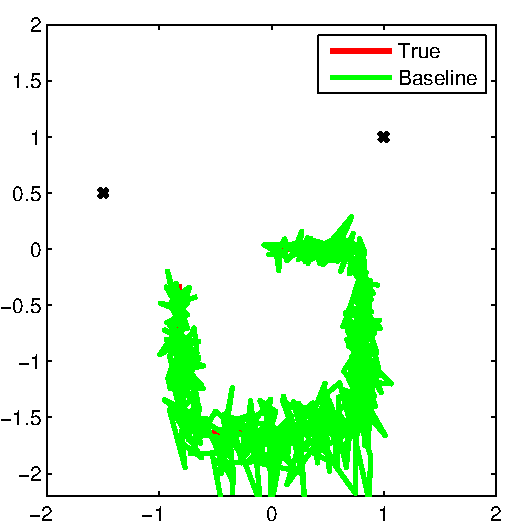
\includegraphics[width=0.7\textwidth]{ex_4_3_baseline}}                
	  \subfloat[EKF approximation]{\label{fig:ex_4_3_ekf}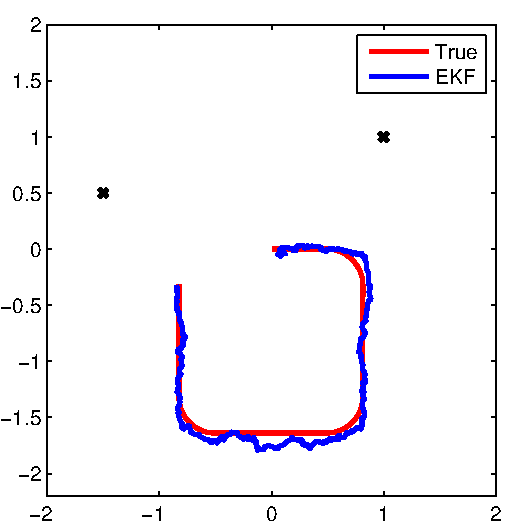
\includegraphics[width=0.7\textwidth]{ex_4_3_ekf}}
  \end{adjustwidth}
  	  \caption{The true trajectory, the baseline approximation and the EKF approximation in exercise~\ref{sec:4_3a}}
	  \label{fig:ex_4_3}
\end{figure}



\begin{table}[h]
	\centering
	\topcaption{The RMSE values in exercise \ref{sec:4_3a}}
	\begin{tabular}{rd{1}{2}d{1}{2}}
\toprule
&\multicolumn{1}{c}{{\bfseries Baseline}}&\multicolumn{1}{c}{{\bfseries EKF}}\\\otoprule
{\bfseries RMSE}&$1.01896$&$0.44085$\\
\bottomrule\end{tabular}

	\label{table:rmse4_3}
\end{table}

\clearpage


\lstinputlisting[linerange=146-208,caption={m-code in exercise~\ref{sec:4_3a}},label=lst:4_3a]{angle_ex.m}

\section{}

\subsection{}\label{sec:5_1}

Here we implement the unscented Kalman filter for the problem in exercise \ref{sec:4_1}
The graphical results are presented in figure \ref{fig:ex_5_1}, where the UKF solution
is compared with the EKF solution, and the mcode in shown listing~\ref{lst:5_1}. With
the chosen parameter values the UKF and SLF solutions become identical and so the RMSE's
are also identical.

\placefig[p]{ex_5_1}{1.0}{The true signal and the EKF and UKF approximations
in exercise~\ref{sec:5_1}}


\clearpage

\lstinputlisting[linerange=89-120,caption={m-code in exercise~\ref{sec:5_1}},label=lst:5_1]{ex4_1.m}




\subsection{}\label{sec:5_2}

Here also the Gauss-Hermite Kalman filter (GHKF) and the cubature Kalman filter (CKF)
were implemented for the previous problem. The solutions of these methods were
identical no matter what the order of the polynomial chosen for GHKF. The solutions
are also identical to the UKF (with the chosen parameters) and SLF solutions. The mcode
is presented in listing~\ref{lst:5_2}.

\lstinputlisting[linerange=130-194,caption={m-code in exercise~\ref{sec:5_2}},label=lst:5_2]{ex4_1.m}


\subsection{}\label{sec:5_3}

Here we implement the UKF and the CKF for the target tracking problem in exercise \ref{sec:4_3}.
Again the parameters for UKF were chosen so that these two methods became identical
The graphical results are presented in figure \ref{fig:ex_5_3}, where the UKF/CKF and EKF solutions
are compared and the mcode in shown listing~\ref{lst:5_3}. The updated RMSE values are presented
in table~\ref{table:rmse5_3}. As can be seen, the CKF/UKF approximation is better but only by a very
slight margin. 

\begin{figure}[htb]
  \begin{adjustwidth}{-2in}{-2in}
	  \centering
	  \subfloat[EKF approximation]{\label{fig:ex_5_3_ekf}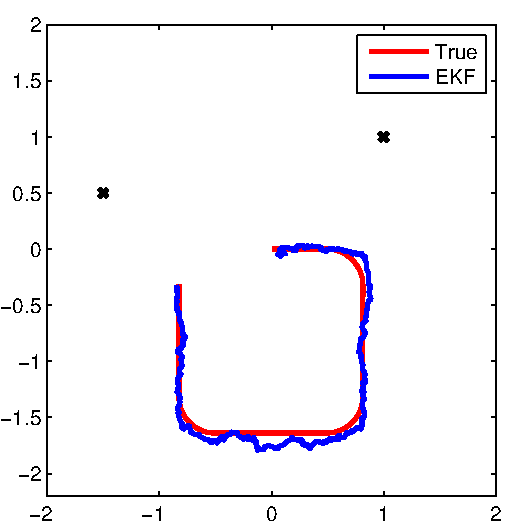
\includegraphics[width=0.7\textwidth]{ex_4_3_ekf}}                
	  \subfloat[CKF/UKF approximation]{\label{fig:ex_5_3_ckfukf}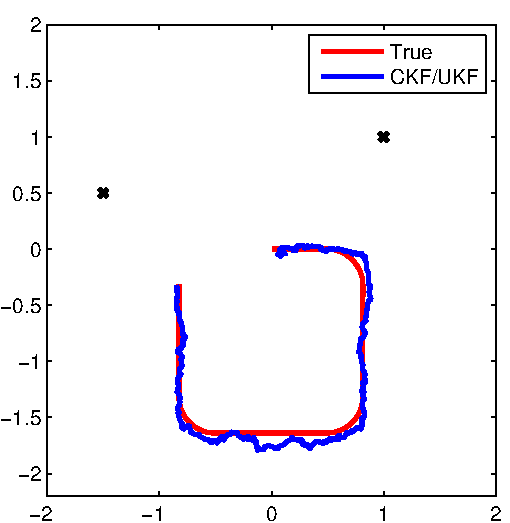
\includegraphics[width=0.7\textwidth]{ex_5_3_ckfukf}}
  \end{adjustwidth}
  	  \caption{The true trajectory, the EKF approximation and the CKF/UKF approximation in exercise~\ref{sec:5_3}}
	  \label{fig:ex_5_3}
\end{figure}


\begin{table}[h]
	\centering
	\topcaption{The RMSE values in exercise \ref{sec:5_3}}
	\begin{tabular}{c c c}
		\otoprule
		Baseline & EKF & CKF/UKF\\
		\midrule
		$1.019$ & $0.441$ & $0.438$\\
		\bottomrule
	\end{tabular}
	\label{table:rmse5_3}
\end{table}


\clearpage

\lstinputlisting[linerange=210-292,caption={m-code in exercise~\ref{sec:5_3}},label=lst:5_3]{angle_ex.m}

\section{}
\subsection{}


\subsection{}\label{sec:6_2}

Here we implement the Bootstrap and sequential importance resampling (SIR) particle filters 
for the problem in exercise \ref{sec:4_1}. Both of the filters were run with $n=700$ particles and
the UKF filter was used in SIR to provide importance distribution.
The graphical results are presented in figure \ref{fig:ex_6_2} and the
mcode in shown listing~\ref{lst:6_2}. The RMSE values are presented in table~\ref{table:rmse6_2}. As can be seen
from the figure and the RMSE table, the SIR filter is somewhat better as was expected.

\placefig[p]{ex_6_2}{1.0}{The true signal and the Bootstrap and SIR approximations
in exercise~\ref{sec:6_2}}


\begin{table}[h]
	\centering
	\topcaption{The RMSE values in exercise \ref{sec:6_2}}
	\begin{tabular}{c c c}
		\otoprule
		Bootstrap & SIR\\
		\midrule
		$0.388$ & $0.355$\\
		\bottomrule
	\end{tabular}
	\label{table:rmse6_2}
\end{table}

\clearpage

\lstinputlisting[linerange=208-300,caption={m-code in exercise~\ref{sec:6_2}},label=lst:6_2]{ex4_1.m}

\subsection{}\label{sec:6_3}

Here we implement the bootstrap filter and SIR with CKF importance distribution for the target tracking problem in
exercise \ref{sec:4_3}. The graphical results are presented in figure \ref{fig:ex_6_3}, where the UKF/CKF and EKF solutions
are compared and the mcode in shown listing~\ref{lst:6_3}. The updated RMSE values are presented
in table~\ref{table:rmse6_3}. As can be seen, the CKF/UKF approximation is better but only by a very
slight margin. 

\begin{figure}[htb]
  \begin{adjustwidth}{-2in}{-2in}
	  \centering
	  \subfloat[Bootstrap
	  approximation]{\label{fig:ex_6_3_bootstrap}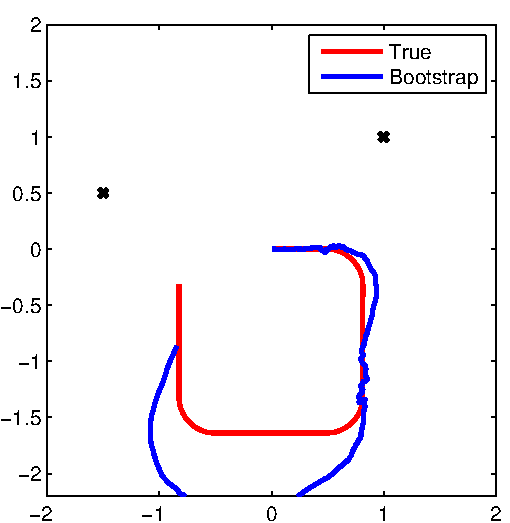
\includegraphics[width=0.7\textwidth]{ex_6_3_bootstrap}}
	  \subfloat[SIR approximation]{\label{fig:ex_6_3_sir}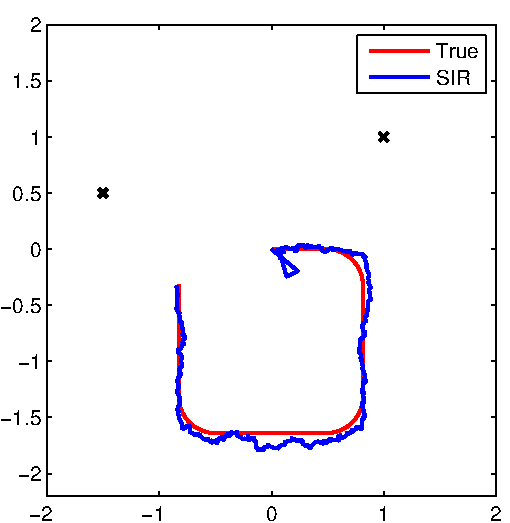
\includegraphics[width=0.7\textwidth]{ex_6_3_sir}}
  \end{adjustwidth}
  	  \caption{The true trajectory, the bootstrap approximation and the SIR approximation in exercise~\ref{sec:6_3}}
	  \label{fig:ex_6_3}
\end{figure}


\begin{table}[h]
	\centering
	\topcaption{The RMSE values in exercise \ref{sec:6_3}}
	\begin{tabular}{c c c}
		\otoprule
		Bootstrap & SIR\\
		\midrule
		$0.946$ & $0.440$\\
		\bottomrule
	\end{tabular}
	\label{table:rmse6_3}
\end{table}


\lstinputlisting[linerange=294-386,caption={m-code in exercise~\ref{sec:6_3}},label=lst:6_3]{angle_ex.m}

\section{}

\subsection{}
\subsubsection{}\label{sec:7_1a}
Here we have implemented the RTS smoother for the random walk model in exercise~\ref{sec:3_2}.
In this simple one dimensional case the RTS smoother equations are given by:
\begin{align}
	G_k &=\frac{P_k}{P_k+Q}\\
	m_k^s&=m_k+G_k\left[m_{k+1}^s-m_k\right]\\
	P_k^s&=P_k+G_k^2\left[P_{k+1}^s-P_{k}-Q\right]
\end{align}

The graphical results of the means are presented in figure~\ref{fig:ex_7_1a_means} and a comparison
of the evolution of the variances of the Kalman filter and the RTS smoother is presented in
figure~\ref{fig:ex_7_1a_variances}. As expected, the RTS smoother variance is smaller in general
and equal to the Kalman filter variance when $k=n$. The m-code is shown in listing~\ref{lst:7_1a}.

\lstinputlisting[linerange=112-129,caption={m-code in exercise~\ref{sec:7_1a}},label=lst:7_1a]{ex3_2.m}

\placefig[p]{ex_7_1a_means}{1.0}{The measurements, the true signal, the Kalman filter solution mean and the RTS smoother
solution mean in exercise~\ref{sec:7_1a}}
\placefig[p]{ex_7_1a_variances}{1.0}{The Kalman filter solution's and the RTS smoother
solution's variances in exercise~\ref{sec:7_1a}}

\subsubsection{}\label{sec:7_1b}
Here the exact smoother of the previous exercise is computed by a grid approximation,
in a similar fashion as for the Kalman filter in exercise~\ref{sec:3_2}. The means and variances
of the smoother and its grid approximation are presented in figures \ref{fig:ex_7_1b_means} and 
\ref{fig:ex_7_1b_variances}. The m-code is shown in listing~\ref{lst:7_1b}.

\lstinputlisting[linerange=158-182,caption={m-code in exercise~\ref{sec:7_1b}},label=lst:7_1b]{ex3_2.m}


\placefig[p]{ex_7_1b_means}{1.0}{The RTS smoother's and its grid approximation's means in exercise~\ref{sec:7_1b}}
\placefig[p]{ex_7_1b_variances}{1.0}{The RTS smoother's and its grid approximation's variances in exercise~\ref{sec:7_1b}}

\subsubsection{}\label{sec:7_1c}
If the stationary Kalman filter is used to provide the filtering distributions for the RTS smoother,
the smoother is supposed to become a stationary backward filter. I have to admit I didn't quite
get this. If an RTS smoother is based on the stationary Kalman filter, the resulting RTS smoother is different
from a smoother where $G=\lim_{k\to\infty}G_k$. Here I choose to use the latter where $G_k=G$, whose
value is taken as the last value from the smoother in \ref{sec:7_1a} (convergence was checked graphically).

In figures \ref{fig:ex_7_1c_means} and \ref{fig:ex_7_1c_variances} the means and variances of the
stationary and non-stationary (the smoother in \ref{sec:7_1a}) smoothers are compared and the m-code
is shown in listing~\ref{lst:7_1c}

\lstinputlisting[linerange=209-223,caption={m-code in exercise~\ref{sec:7_1c}},label=lst:7_1c]{ex3_2.m}

\placefig[p]{ex_7_1c_means}{1.0}{The RTS and the stationary RTS smoother's means in exercise~\ref{sec:7_1c}}
\placefig[p]{ex_7_1c_variances}{1.0}{The RTS and the stationary RTS smoother's variances in exercise~\ref{sec:7_1c}}

\subsection{}\label{sec:7_2}

Here we have implemented the RTS smoother to the resonator model in exercise~\ref{sec:3_3}.
The performances of the base-line, the Kalman filter and the RTS smoother solutions
are presented in table~\ref{table:rmse7_2}.




\placefig[p]{ex_7_2}{1.0}{The Kalman filter's and RTS smoother's means in exercise~\ref{sec:7_2}}

\subsection{}\label{sec:7_3}
\subsubsection{}\label{sec:7_3a}
We proceed in the same fashion as in the derivation of the Kalman filter and the statistically linearized
Kalman filter. The goal is to calculate the smoothing distribution $p(\v{x}_k|\v{y}_{1:T})$, where $T$ is the number
of all the observations, with a recursive formula. Let's assume that we know the Gaussian filtering distributions $p(\v{x}_k|\v{y}_{1:k})=N(\v{x}_k|\v{m}_k,\v{P}_k)$
and that we have a non-linear dynamical model with additive Gaussian noise: $\v{x}_{k+1}=\v{f}(\v{x}_{k})+\v{q}_{k}$. Now taking
into account the assumed Markov properties, we get
\begin{align}
	p(\v{x}_k,\v{x}_{k+1}|\v{y}_{1:k})&=p(\v{x}_{k+1}|\v{x}_k)p(\v{x}_k|\v{y}_{1:k}).
\end{align}
To make this joint distribution Gaussian, we can apply the statistical linearization based Gaussian approximation, giving
\begin{align}
	p(\v{x}_k,\v{x}_{k+1}|\v{y}_{1:k})&=
	N\left(
	\begin{bmatrix}
		\v{x}_k\\\v{x}_{k+1}
	\end{bmatrix}\left\vert
	\begin{bmatrix}
		\v{m}_{k}\\
		\v{m}_{k+1}^-
	\end{bmatrix}
	\right.,
	\textrm{diag}\left(
	\begin{bmatrix}
		\v{m}_{k}\\
		\v{P}_{k+1}^-
	\end{bmatrix}
	\right)\right)
\end{align}
Taking the marginal distribution of $\v{x}_{k+1}$ gives the prediction
equations that I will present in the end. Taking again into account
the conditional independence properties of the Markov chain we see that
$p(\v{x}_k|\v{x}_{k+1},\v{y}_{1:T})=p(\v{x}_k|\v{x}_{k+1},\v{y}_{1:k})$ which is given by the 
conditional distribution lemma of a joint normal distribution. Then
\begin{align}
	p(\v{x}_k,\v{x}_{k+1}|\v{y}_{1:T})&=p(\v{x}_k|\v{x}_{k+1},\v{y}_{1:k})p(\v{x}_{k+1}|\v{y}_{1:T}),
\end{align}
where $p(\v{x}_{k+1}|\v{y}_{1:T})$ is the smoothing distribution of the previous step,
is again joint normal, so that $p(\v{x}_k|\v{y}_{1:T})$ is given by the marginal
distribution formula for the joint normal distribution. Putting all this together
and using the matrix inversion lemma we get:

\begin{align}
	\shortintertext{prediction:}
	\v{m}_{k+1}^-&=\E{\v{f}(\v{x}_{k})}\\
	\v{P}_{k+1}^-&=\E{\v{f}(\v{x}_{k})\delta \v{x}_k^T}\v{P}_{k}^{-1}\E{\v{f}(\v{x}_{k})\delta \v{x}_k^T}^T+\v{Q}_k
	\shortintertext{update:}
	\v{G}_k&=\E{\v{f}(\v{x}_{k})\delta \v{x}_k^T}^T\left[\v{P}_{k+1}^-\right]^{-1}\\
	\v{m}_k^s&=\v{m}_k+\v{G}_k\left[\v{m}_{k+1}^s-\v{m}_{k+1}^-\right]\\
	\v{P}_k^s&=\v{P}_k+\v{G}_k\left[\v{P}_{k+1}^s-\v{P}_{k+1}^-\right]
\end{align}

 


\subsubsection{}\label{sec:7_3b}
Here we have implemented the statistically linearized RTS smoother and the
extended RTS smoothers for the problem in exercise~\ref{sec:4_1}. Graphical comparison
of the implemented filters and smoothers is presented in figure~\ref{fig:ex_7_3} and
the RMSE's are compared in table~\ref{table:rmse7_3}.

\begin{table}[h]
	\centering
	\topcaption{The RMSE values in exercise \ref{sec:7_3}}
	\begin{tabular}{c c c c}
		\otoprule
		EKF & SLF & ERTS & SLRTS\\
		\midrule
		$0.946$ & $0.440$ & $0.946$ & $0.440$\\
		\bottomrule
	\end{tabular}
	\label{table:rmse7_3}
\end{table}


\placefig[p]{ex_7_3}{1.0}{The RTS smoothers for the EKF (ERTS) and SLF (SL RTS) filters in exercise~\ref{sec:7_3}}

\subsubsection{}\label{sec:7_3c}

This is analogical to exercise~\ref{sec:4_2c}:

\begin{align}
	\shortintertext{prediction:}
	\v{m}_{k+1}^-&=\E{\v{f}(\v{x}_{k})}\\
	\v{P}_{k+1}^-&=\E{\v{F}_{\v{x}}(\v{x}_{k})}\v{P}_{k}^{T}\E{\v{F}_{\v{x}}(\v{x}_{k})}^T+\v{Q}_k
	\shortintertext{update:}
	\v{G}_k&=\E{\v{F}_{\v{x}}(\v{x}_{k})}^T\left[\v{P}_{k+1}^-\right]^{-1}\\
	\v{m}_k^s&=\v{m}_k+\v{G}_k\left[\v{m}_{k+1}^s-\v{m}_{k+1}^-\right]\\
	\v{P}_k^s&=\v{P}_k+\v{G}_k\left[\v{P}_{k+1}^s-\v{P}_{k+1}^-\right]
\end{align}



%\bibliographystyle{plain}
%\bibliography{viitteet}
\end{document}
